\section{Introduction}
\label{sec:introduction}

Logicians must be familiar with \emph{modus ponens}, $ A \ta B, A \vdash B $, a very common rule of inference, stating that given implication $ A \ta B $ and proposition $ A $, one can conclude $ B $. Programmers may frequently use \emph{function application}: if $ f $ is a function of type $ A \ta B $ and $ x $ is an argument of type $ A $, then the application $ f x $ has type $ B $. Interestingly, modus ponens behaves the same as function application. It seems that proofs should be related to programs. Indeed, there is a precise correspondence between them, which is known as the Curry-Howard Isomorphism \cite{Mit96,SU98}.

In the 1930s, Haskell Curry observed a correspondence between types of combinators and propositions in intuitionist implicational logic. But, at that time, it was viewed as no more than a curiosity. About three decades later, William Howard extended this correspondence to first order logic by introducing dependent types. As a result, this correspondence is called the Curry-Howard Isomorphism \cite{Hin97}.

The Curry-Howard Isomorphism states a correspondence between systems of formal logic and computational calculi. It has been extended to more expressive logics, e.g. higher order logic, and other mathematical systems, e.g. cartesian closed categories. In this project, I mainly probed into one of its extensions, the three-way correspondence between intuitionistic propositional logic, simply-typed lambda calculus and cartesian closed categories, with propositions or types being interpreted as objects and proofs or terms as morphisms \cite{AL91,LS86,Mit96,Pit00}.

\begin{center}
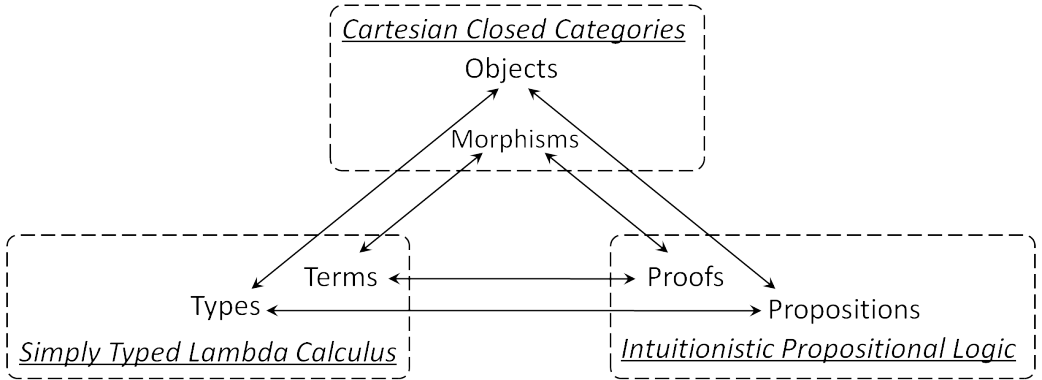
\includegraphics[width=0.9\textwidth]{./images/triangle}
\end{center}

Intuitionistic logic is a formalisation of Brouwer’s intuitionism. As the founder of intuitionism, L. E. J. Brouwer avoided use of formal language or logic all his life. But his attitude did not stop others considering formalisations of parts of intuitionism. In the 1930s, Arend Heyting, a former student of Brouwer, produced the first complete axiomatisations for intuitionistic propositional and predicate logic \cite{Rui91}. In intuitionistic logic, \emph{reductio ad absurdum} is not a rule; therefore, neither of the law of excluded middle and double negation elimination is provable.

The lambda calculus was introduced by Alonzo Church in the early 1930s as a formal system to provide a functional foundation for mathematics \cite{Bar85,Hin97}. Since Church's original system was shown to be logically inconsistent, he gave just a consistent subtheory of his original system dealing only with the functional part. Then, in 1940, Church also introduced a typed interpretation of the lambda calculus by giving each term a unique type. Today, the typed lambda calculus serves as the foundation of the modern type systems in computer science.

Categories first appeared in Samuel Eilenberg and Saunders Mac Lane's paper \cite{SS45} written in 1945. It was originally introduced to describe the passage from one type of mathematical structure to another. In recent decades, category theory has found use for computer science. For instance, it has a profound influence on the design of functional and imperative programming languages, e.g. Haskell and Agda.

Looking from the historical perspective, these three diverse systems seem to have different origins, not related to each other. However, Joachim Lambek showed in the early 1970s that cartesian closed categories provided a formal analogy between proofs in intuitionistic propositional logic and types in combinatory logic \cite{Lam72}. As a result, some people may use Curry-Howard-Lambek Isomorphism to refer to this three-way correspondence.